\section{Aufbau}
\label{sec:Aufbau}

Um die Suszeptibilität eines Materials zu ermitteln, kann ausgenutzt werden, dass sich die Induktivität $L$ einer Spule ändert, falls Materie in diese eingeführt wird. Es gilt:
\begin{equation}
	\Delta L = \mu_0 \chi Q \frac{n^2}{l}=\chi L \frac{Q}{F}\text{,}
\end{equation}
wobei $Q$ die Querschnittsfläche der Probe, $F$ die Querschnittsfläche und $l$ die Länge der Spule ist. Um diese kleinen Änderungen messen zu können kann eine Brückenschaltung gemäß Abbildung \ref{fig:Brückenschaltung} verwendet werden.
\begin{figure}
	\centering
	\caption{Eine mögliche Brückenschaltung zur Messung der Suszeptibilität von Stoffen.}
	\includegraphics[width=\linewidth-70pt,height=\textwidth-200pt,keepaspectratio]{content/images/Brückenschaltung.png}
	\label{fig:Brückenschaltung}
\end{figure}
Für den Betrag der Brückenspannung $U_\text{Br}$ gilt dann:
\begin{equation}
	U_\text{Br} = w \Delta L \frac{U_\text{Sp}}{4 \sqrt{R^2+w^2+L^2}}
\end{equation}
mit der Winkelgeschwindigkeit $w$. Umgestellt nach $\chi$ und in Näherung für große Frequenzen ergibt sich:
\begin{equation}
	\chi\approx 4\frac{F U_\text{Br}}{Q U\text{Sp}}\text{.}\label{eq:SusU}
\end{equation}
Auch kann die Brückenschaltung nach dem Einführen des Materials erneut abgeglichen werden und es ergibt sich $R'_3 = R_3 + \Delta R_3 $ mit $\Delta R_3 = \chi \frac{R_3 Q}{2 F}$ oder auch umgestellt:
\begin{equation}
	\chi = \frac{2 \Delta R_3 F}{R_3 Q}\text{.}\label{eq:SusR}
\end{equation}
\begin{figure}
	\centering
	\caption{Eine Schaltskizze von einem möglichen Aufbau zur Messung der Suszeptibilität von Stoffen.}
	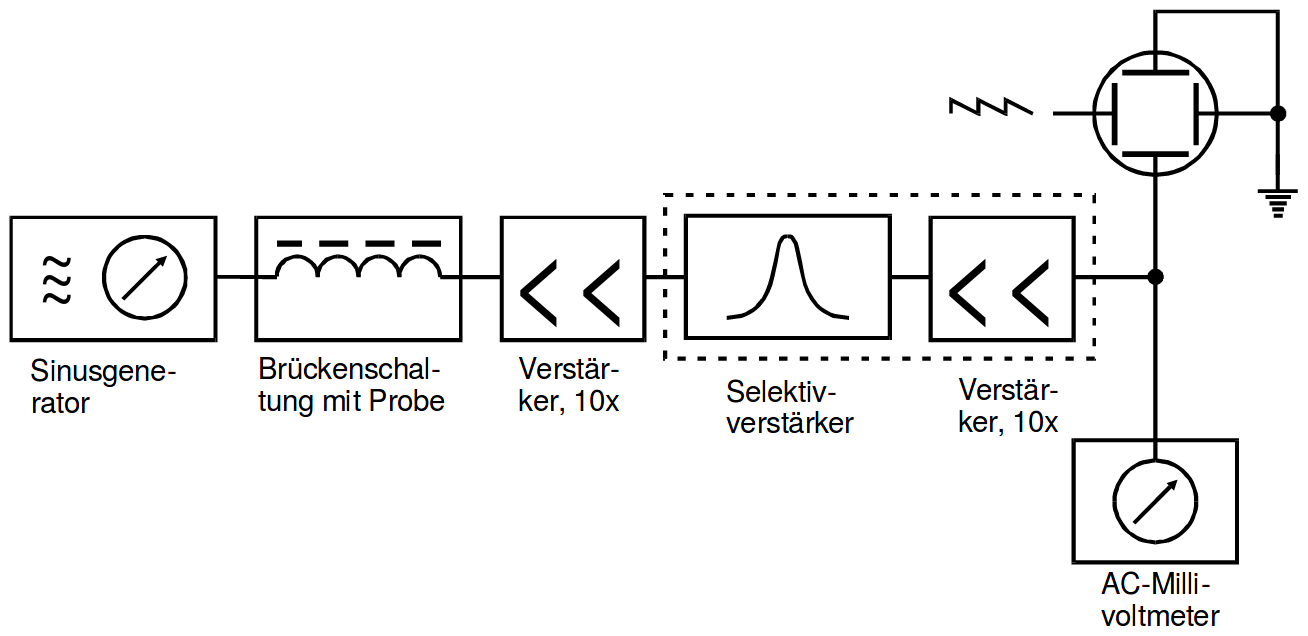
\includegraphics[width=\linewidth-70pt,height=\textheight-70pt,keepaspectratio]{content/images/Schaltskizze.png}
	\label{fig:Schaltskizze}
\end{figure}
Jedoch treten viele Störspannungen bei dieser Messmethode auf. Diese müssen herausgefiltert werden. Hierfür wird ein Selektivverstärker gewählt der besonders gut die Frequenz des Sinusgenerators durchlässt. Dieser wird zwischen der Schnittstelle der Brückenspannung und dem AC-Millivoltmeter gemäß Abbildung \ref{fig:Schaltskizze} angeschlossen.
